\begin{figure}
\centering
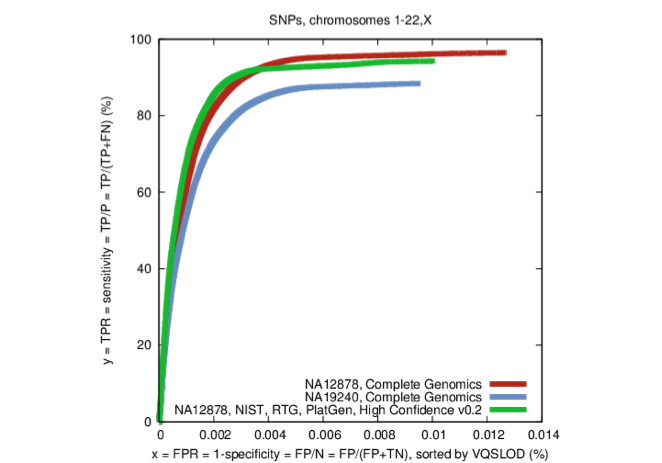
\includegraphics[width=0.8\textwidth]{fig/SN09f2}
\caption[\Gls{ROC} curve]{\gls{ROC} curve of low coverage \gls{WGS} data for NA12878 and NA19240 compared to 30x coverage sequencing for different \gls{VQSLOD} filtering scores. On the x-axis is the \gls{FPR} (1-specificity) and on the y-axis is the \gls{TPR} (sensitivity) with respect to the highly curated high coverage genomes from these individuals. The green curve represents the sensitivity and specificity of 4x sequence data for NA12878 in comparison with gold standard data within high confidence intervals. The red and blue lines represent these parameters calculated across the genome for NA12878 and NA19240. We find that the sensitivity for the NA19240 sample is less than that of the NA12878, which probably reflects the fact, that the African sample contains a greater number of singletons than NA12878 relative to the 3 sequenced populations. Each point on the monotonic curve corresponds to the sensitivity and specificity obtained at a particuar VQSLOD threshold used for filtering. The truth sensitivity threshold is itself a monotonic function of the VQSLOD score. We find that the highest sensitivity and specificity for the highly confident sites (green line) corresponds to a GATK \gls{VR} truth sensitivity threshold of 99\%.}
\label{fig:SN09f2}
\end{figure}